\documentclass[a4paper, 12pt]{article}

% This file contains global setup commands so that we can write in our main document without cluttering up the workspace. This file is the first thing included in the main paper after the \documentclass command, and all settings are immediately available.

\usepackage{graphicx}
\usepackage{xcolor}
\usepackage{parskip}
\usepackage{wrapfig}
\usepackage{amsmath}

% Font settings
\usepackage{fontspec}
\usepackage{titlesec}
\usepackage{titling}
\setmainfont{Open Sans}
\newfontfamily \headingfont[]{Open Sans Light}
\newfontfamily \codefont[NFSSFamily=JetBrainsMono]{JetBrains Mono}
\definecolor{accent}{rgb}{0.8, 0.0, 0.0}
\titleformat{\section}
	{\Huge\headingfont}{\thesection}{1em}{}[{\color{accent}\titlerule[4pt]}]
\titleformat{\subsection}
	{\Large\headingfont}{\thesection}{1em}{}[{\color{accent}\titlerule[2pt]}]
\titleformat{\subsubsection}
	{\large\headingfont}{\thesection}{1em}{}[{\color{accent}\titlerule[1pt]}]
\setmonofont{JetBrains Mono}
% Set to clear page before each section.
\newcommand{\sectionbreak}{\clearpage}

% Link settings
\usepackage{hyperref}
\definecolor{linkcolour}{rgb}{0.7, 0.133, 0.133}
\hypersetup{
	colorlinks,
	breaklinks,
	urlcolor=linkcolour,
	linkcolor=linkcolour,
	citecolor=linkcolour
}

% Code settings
\usepackage{minted}
\usepackage[htt]{hyphenat}

% Note: For some reason, this patch is needed to allow minted to work with python3, since it just looks for "python" by default.
\usepackage{xpatch}
\makeatletter
\xpatchcmd\minted@pygmentize
	{python -c}
	{python3 -c}
	{}{\fail}
\xpatchcmd\minted@autogobble
	{python -c}
	{python3 -c}
	{}{\fail}
\makeatother

\usemintedstyle{default}
\definecolor{codebg}{rgb}{0.973, 0.973, 0.973}
\definecolor{codehighlight}{rgb}{0.360, 0.215, 0.309}
\setminted{
	autogobble=true,
	encoding=utf-8,
	numbers=left,
	bgcolor=codebg,
	highlightcolor=codehighlight,
	fontfamily=JetBrainsMono,
	fontsize=\scriptsize,
	breaklines,
	tabsize=2
}
\renewcommand{\theFancyVerbLine}{\sffamily{\scriptsize\oldstylenums{\arabic{FancyVerbLine}}}}

% Header/Footer settings
\usepackage{fancyhdr}
\usepackage{lastpage}
\usepackage[left=3cm, right=3cm, top=2cm, bottom=4cm]{geometry}
\pagestyle{fancy}
\fancyhead[L,C,R]{}
\renewcommand{\headrulewidth}{0pt}
% Footer definition
\fancyfoot[L]{
	
\includegraphics[width=2cm]{img/rug_icon.jpg}
}
\fancyfoot[C]{}
\fancyfoot[R]{
	\headingfont
	\large
	Page \thepage\ of \pageref*{LastPage}
	\normalfont
	\normalsize
}

% Bibiliography settings
\usepackage[
	backend=bibtex,
	style=numeric,
	natbib=true,
	autocite=superscript
]{biblatex}
\addbibresource{sources.bib}

\setcounter{secnumdepth}{-3}

\begin{document}

% This file defines the title page formatting.

\begin{titlepage}
	\headingfont
	\begin{center}
		\LARGE \textbf{On the Efficacy of Keyword Searches to Find Meaningful Architectural Knowledge in Open-Source Software Mailing Lists}
		
		\vspace{0.5cm}
		
		\Large
		Bachelor Thesis for Computing Science
		
		\vspace{2cm}
		
		\begin{tabular}{l r}
			\Large \textbf{Andrew Lalis} & \footnotesize\href{mailto:andrewlalisofficial@gmail.com}{andrewlalisofficial@gmail.com} \\
			\footnotesize Supervised by \normalsize\textbf{Dr. Mohamed Soliman} & \footnotesize\href{mailto:m.a.m.soliman@rug.nl}{m.a.m.soliman@rug.nl}
		\end{tabular}
		
		
		\vspace{1cm}
		
		\small
		\normalfont
		\today
		
		\vfill
				
		
\includegraphics[width=\textwidth]{img/rug_fse_logo.png}
	\end{center}

	% Reset settings after we're done.
	\normalfont
	\normalsize
\end{titlepage}

\section{Abstract}
	This section will contain a brief overview of the research and conclusions. Test

{% Use a separate format for the table of contents.
	\hypersetup{linkcolor=black}
	\headingfont
	\tableofcontents
}

\section{Introduction}
	In this paper, we'll explore the efficacy of using targeted keyword search queries to find architectural knowledge in mailing lists for open-source software projects. More simply put, we'll build tools, collect data, and analyze that data to qualitatively determine how effective certain keyword-based search queries are at finding useful information in large sets of emails, sent in mailing lists for developers to communicate about large open-source software projects.
	
	\subsection{Software Architecture}
		Behind every software system you interact with, including the one used to read this paper, is a set of elements, relationships, and rationale that define the software's architecture. While on the surface, you see the \textit{implementation} of the software, the \textit{architecture} is concerned with what elements, their interactions in order to provide a framework for satisfying the requirements of the system \autocite{perry}. Continuing our example, the software you're using to read this paper probably uses an architecture that includes elements like a PDF renderer, file reader, and a controller to manage your button clicks and mouse scrolling. Collectively, this set of components, design decisions, rationale, assumptions, and context together are defined as the \textit{architectural knowledge} of the system\autocite{denboon}.
		
		In Perry's 1992 paper, "Foundations for the Study of Software Architecture", he posits that "we have not yet arrived at the stage where we have a standard set of architectural styles with their accompanying design elements and formal arrangements," and that each system is "a new architecture" \autocite{perry}. While we are perhaps nearer now, 30 years later, to that mythical stage of architectural standardization, indeed many new systems are genuinely new architectures, with new elements or entirely novel approaches to communicating between components, where engineers must consult both their acquired skills and the collective knowledge of their peers, to make a best-effort to build a system to satisfy their requirements.
		
		Despite the plethora of resources available to the modern software engineer, we still often see \textit{architectural knowledge vaporization}\autocite{jansen} because of undocumented decisions engineers took when designing the architecture of a system, or because it's impossible or practically infeasible to extract useful information. This dissipation of knowledge is a function of time and architecture size, and can lead to some serious problems that have already established themselves as hallmarks of poor software design in the industry, such as an increasing cost to improve or upgrade a system \autocite{jansen, perry}, and a lack of reusability \autocite{jansen}, and an increased cost of maintenance \autocite{randell} even when no new features are added. These costs can, and often do, reach a point at which it is simply more effective to start over, abandoning completely any established work on an architecture. Through the years, this evolved from reprogramming low-level batch programs for early computing installations\autocite{randell}, to today's distributed systems. Succinctly, a loss of architectural knowledge, by conjecture, leads to a loss of value and a loss of efficiency, and this paper aims to add additional tools to our collective defense against such regression.
		
	\subsection{Searching}
		\textbf{TODO: Add more background about what searching has been done already, what possibilities there are.}
	
		It is important to explore different avenues for acquiring knowledge, especially as the body of information grows exponentially with time. It is difficult for developers and software architects to make informed decisions about their own projects, because the source of their knowledge is distributed in a variety of disparate sources. If we can reliably glean information about software architecture and the successful (and unsuccessful) decisions that other field experts have made, we can make this knowledge more accessible for all.
		
	\subsection{Research Questions}
		The main research question that this paper attempts to answer is summarized in the following question:
		
		\large \textbf{What architectural knowledge exists in open-source software development mailing lists?}
		\normalsize
		
		In addition to the main question we're attempting to answer, this paper will also discuss several other possible questions and answers that may be obtained using the data originally gathered for the main question.
		
		\begin{enumerate}
			\item Does there exist a relationship in the order in which architectural decisions are discussed, chronologically in an email thread? Is there significance in the order in which architectural decisions are made?
			
			\item Is there a relationship between the content of discussion in emails, and related issues in issue/ticket boards such as \href{https://www.atlassian.com/software/jira}{JIRA} and \href{https://github.com/features/issues}{GitHub issues}?
			
			\item How can we use data gathered in this research to improve our search queries?
		\end{enumerate}
	
\section{Related Work}
	This section will contain an overview of lots of different sources and what they've done, and how what I'm doing is different.

\section{Methodology}
	For the purposes of this research, we will focus on analyzing the contents of mailing lists from three major open-source projects from the Apache Software Foundation: \href{https://hadoop.apache.org/}{Hadoop}, \href{https://cassandra.apache.org}{Cassandra}, and \href{https://attic.apache.org/projects/tajo.html}{Tajo}. Mailing list data will be obtained from \href{https://lists.apache.org/}{lists.apache.org}, and this data will be indexed and searched over using \href{https://lucene.apache.org/}{Apache Lucene}. A subset of emails from these mailing lists will be categorized based on the type of architectural design decisions they contain, in order to conjecture about the efficacy of searching.
	
	\footnotesize
	Note: All software and components developed for this research are available on GitHub.com under the \href{https://github.com/ArchitecturalKnowledgeAnalysis}{ArchitecturalKnowledgeAnalysis} organization. All software is licensed under the permissive \href{https://en.wikipedia.org/wiki/MIT_License}{MIT license}, and may be freely used or redistributed however you see fit.
	\normalsize
	
	\subsection{Choosing Sources}
		While previous work by den Boon chose to analyze data from both issue tracking boards and mailing lists from open-source software projects\autocite{denboon}, this research will limit the scope of sources to just mailing lists, since that is the focus of our research questions. More specifically, a \textit{mailing list} is a "mechanism whereby a message may be distributed to multiple recipients by sending to one address."\autocite{mailinglistrfc} Put more plainly, someone may \textit{subscribe} to a mailing list, and in doing so, they will receive any email which is addressed to that list. Likewise, that person may also send an email to the list's address, and it will be broadcast to all other subscribed recipients. In the context of software development, mailing lists have been used extensively since their inception as a way to collectively discuss and make design decisions regarding large open-source projects. Because of this, we can expect mailing lists for software development to be particularly rich in architectural knowledge, and they make a good candidate for analyzing the effectiveness of various search approaches.
		
		Within the domain of mailing list communications, we can further narrow our search down to software projects which we can reasonably expect to contain a large amount of, and large variety of architectural decisions. These would generally be large projects with many moving parts, which have a broad range of applications and societal uses. The Apache Software Foundation (ASF) is a leader in these sorts of projects, with many open-source systems for managing, processing, and searching through big data, which find their usage in various state-of-the-art enterprises and research endeavors, notably NASA, Facebook, Twitter, Netflix, and so on\autocite{akhtar}. From the ASF, we chose mailing lists from the following three projects for analysis:
		
		\begin{enumerate}
			\item \href{https://cassandra.apache.org}{Cassandra} - An open source NoSQL distributed database trusted by thousands of companies for scalability and high availability without compromising performance.
			\item \href{https://hadoop.apache.org/}{Hadoop} - A framework that allows for the distributed processing of large data sets across clusters of computers using simple programming models. It is designed to scale up from single servers to thousands of machines, each offering local computation and storage.
			\item \href{https://tajo.apache.org/}{Tajo} - A robust big data relational and distributed data warehouse system for Apache Hadoop. Tajo is designed for low-latency and scalable ad-hoc queries, online aggregation, and ETL (extract-transform-load process) on large-data sets stored on HDFS (Hadoop Distributed File System) and other data sources.
		\end{enumerate}
		
		\footnotesize Project descriptions obtained from the respective projects' homepages.
		\normalsize
		
		For each of the above projects, we obtained one or more mailing lists dedicated to the discussion of the project's internal development, thus excluding irrelevant discussions about usage and user issue reports.
		
		For Cassandra, we chose the following mailing lists:
		\begin{itemize}
			\item \href{https://lists.apache.org/list.html?dev@cassandra.apache.org}{dev@cassandra.apache.org}
		\end{itemize}
	
		For Hadoop, we chose the following mailing lists:
		\begin{itemize}
			\item \href{https://lists.apache.org/list.html?common-dev@hadoop.apache.org}{common-dev@hadoop.apache.org}
			\item \href{https://lists.apache.org/list.html?hdfs-dev@hadoop.apache.org}{hdfs-dev@hadoop.apache.org}
			\item \href{https://lists.apache.org/list.html?mapreduce-dev@hadoop.apache.org}{mapreduce-dev@hadoop.apache.org}
			\item \href{https://lists.apache.org/list.html?yarn-dev@hadoop.apache.org}{yarn-dev@hadoop.apache.org}
		\end{itemize}
	
		For Tajo, we chose the following mailing lists:
		\begin{itemize}
			\item \href{https://lists.apache.org/list.html?dev@tajo.apache.org}{dev@tajo.apache.org}
		\end{itemize}
	
	\subsection{Fetching and Processing Sources}
		The first step to being able to analyze and identify architectural knowledge in mailing lists is, of course, to obtain the emails from the mailing lists in the first place. For this purpose, the \href{https://github.com/ArchitecturalKnowledgeAnalysis/EmailDownloader}{EmailDownloader} utility library was developed, and for parsing and preparing data for use in our datasets, the \href{https://github.com/ArchitecturalKnowledgeAnalysis/MBoxParser}{MBoxParser} utility library was developed.
		
		\subsubsection{Downloading}
			The EmailDownloader utility offers an asynchronous interface for downloading a series of MBox (email archive format) files to a directory. Because all of the mailing lists used by this research come from the Apache Software Foundation, the library includes an implementation for downloading from the ASF's mailing list internal API at \href{https://lists.apache.org/api/mbox.lua}{https://lists.apache.org/api/mbox.lua}, with support for rate-limited downloading and the ability to detect long periods of inactivity and short-circuit prematurely to save time.
			
			While this library is primarily designed to be included in other Java projects for a complete workflow, it can also be run as a standalone program that offers the same interface on the command-line, if you wish to use it like this.
			
			The end result is that we are able to download a large archive of all emails sent in a mailing list, since its inception, to today.
			
		\subsubsection{Processing}
			Once we have downloaded a large amount of MBox files, we must parse their contents to extract the individual emails for use in our analysis. This is done by the \href{https://github.com/ArchitecturalKnowledgeAnalysis/MBoxParser}{MBoxParser} utility library, which offers an interface for parsing a collection of MBox files and issuing a callback handler for each email that was obtained.
			
			The end result is a collection of many Email objects that are ready for further use, whose format is described in the code snippet below:
			\begin{minted}[linenos=false]{java}
public class Email {
	public String messageId;
	public String inReplyTo;
	public String sentFrom;
	public String subject;
	public ZonedDateTime date;
	
	public String mimeType;
	public String charset;
	public String transferEncoding;
	public byte[] body;
}
			\end{minted}
		
			\footnotesize
			Note that the MBoxParser library performs a few rudimentary operations to attempt to clean up ill-formatted emails. This includes sanitizing various date formats, and stripping superfluous characters from an email's MESSAGE\_ID.
			
			For more details, please see \href{https://github.com/ArchitecturalKnowledgeAnalysis/MBoxParser/blob/main/src/main/java/nl/andrewl/mboxparser/EmailContentHandler.java}{nl.andrewl.mboxparser.EmailContentHandler}.
			\normalsize
			
	\subsection{Dataset Format}
		Once a sufficient number of emails have been downloaded as described in the previous section, they can be ingested by the \href{https://github.com/ArchitecturalKnowledgeAnalysis/EmailIndexer}{EmailIndexer} API to generate a \textit{dataset}. This dataset is simply a directory containing the following components:
		
		\begin{enumerate}
			\item An embedded relational \href{https://www.h2database.com}{H2 database} file named \texttt{database.mv.db}, which stores all emails, tags, and other key information for the dataset. A \hyperref[fig:schema]{schema diagram} is provided in this section, and the full schema definition can be found \hyperref[sec:dataset-schema]{in the appendix}.
			\item An \texttt{index} directory in which the indexes generated by \href{https://lucene.apache.org/}{Apache Lucene} are stored.
			\item A \texttt{metadata.properties} file that holds some meta information about the dataset. As of the time of writing, the only metadata stored in this file is the dataset version, which, again at the time of writing, is version 2.
		\end{enumerate}
	
		\subsubsection{Database Schema}
			\begin{wrapfigure}{r}{0.5\textwidth}
				\label{fig:schema}
				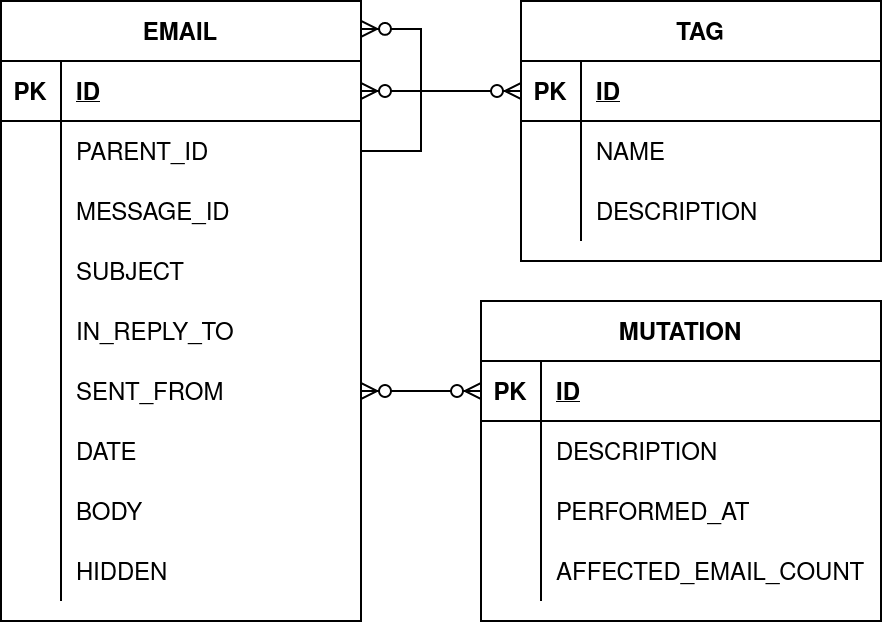
\includegraphics[width=0.5\textwidth]{img/simple_schema.png}
				\caption{A diagrammatic representation of the email dataset's relational schema.}
			\end{wrapfigure}
			The relational schema is the core of the email dataset, and defines how we operate on and organize the data. It is purposefully designed to be as simple as possible, to make it easy to use the dataset in a variety of applications and environments.
			
			The schema consists of three entities: \textit{emails}, \textit{tags}, and \textit{mutations} (although mutations are not strictly required).
			
			\textbf{Emails} are, as you'd probably expect, the entity that represents a single email message, sent by someone, in a mailing list. While emails \textit{do} have their own unique \texttt{MESSAGE\_ID} attribute\autocite{rfc5322}, they are identified by an 8-byte integer primary key. This reduces the dataset size, improves search performance due to the monotonic nature of incrementing primary keys, and allows for easier referencing of emails by their id, instead of a long, randomly-generated message id.
			
			Also of note is an email's \texttt{PARENT\_ID}, which is a self-referencing foreign key that references another email entity by its id. This foreign key is the manifestation of the \textit{many-to-one} relationship between an email and its parent, where many "child" emails may refer to one parent email. The parent id is derived, when processing emails, from the email's "In-Reply-To" field. According to RFC 5322, the in-reply-to field, if present, must reference another email's message-id, and this format of replies forms the basis of an email thread's structure\autocite{rfc5322}.
			
			\textbf{Tags} are entities which can be attached to any number of emails, to offer a method of categorizing emails. Originally in version 1 of the dataset format, tags were not entities but simple texts that were attached to each email, but it was discovered during the development of the tools for this research that there are several benefits to having tags as their own entities: the ability to edit a tag's name, provide a description, and reduce the total dataset size by referencing an 4-byte integer id instead of keeping a copy of a string for each tag applied to an email.
			
			There exists a \textit{many-to-many} relationship between \textbf{emails} and \textbf{tags}, which one could verbalize as, "A tag may be applied to many emails, and an email may have many tags applied to it."
			
			\textbf{Mutations} are entities that record some change to the dataset which is used as a historical record of how a the emails in a dataset are filtered or modified. Mutations are used at the discretion of any third-party application which interfaces with the EmailIndexer API, and are not required to be used.
			
			There exists a \textit{many-to-many} relationship between \textbf{mutations} and \textbf{emails}, which one could verbalize as, "A mutation may involve many emails, and an email may be involved in many mutations." It is not required that a mutation be linked to any emails.
			
		\subsubsection{Indexing with Lucene}
			Alongside the relational database resides the \texttt{index} directory, as mentioned at the start of this section. This contains the indexes produced by the \href{https://lucene.apache.org/}{Apache Lucene} indexing library when we build an index using the emails in the database. This index is then used for executing query searches over the database by users.
			
			For each email in the dataset, we index the following fields as non-stored string-type fields using the \texttt{DOCS\_AND\_FREQS\_AND\_POSITIONS} index options provided by Lucene\autocite{apache-lucene}:
			\begin{itemize}
				\item The \texttt{SUBJECT} field.
				\item The \texttt{BODY} field.
			\end{itemize}
			In addition to these indexed fields, we store the email's id and pre-compute the \textit{root id} (id of the first email in the current email's thread), as these are essential for producing actionable results from any query search on the index.
			
	\subsection{Email Thread Structure}
		\begin{wrapfigure}{r}{0.4\textwidth}
			\label{fig:email-threads}
			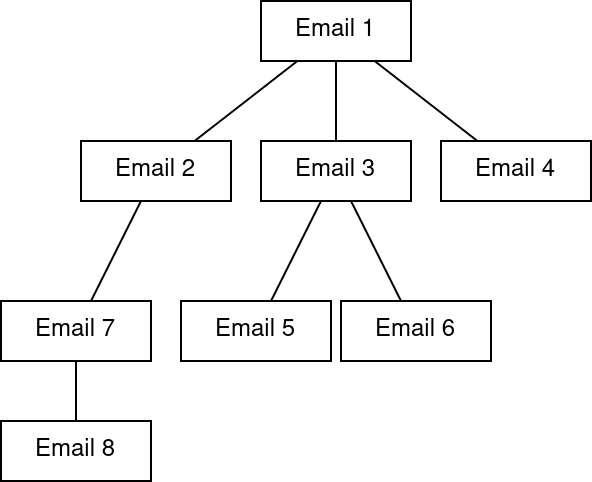
\includegraphics[width=0.4\textwidth]{img/email-threads.png}
		\end{wrapfigure}
	
		As previously mentioned, emails have a self-referencing \textit{many-to-one} relationship defined by their "In-Reply-To" field. It is important to understand the consequences of this structure, and how it impacts the dynamics of processing data. In any information system, a self-referencing, many-to-one relationship that an entity participates in, can be interpreted as a \textit{tree} data structure.
	
		Each email can be thought of as a node in the tree, where each reply to that email forms a branch. There is no limit to how wide or deep the tree can become, because there is no universal hard limit on the number of replies to an email, nor on how many replies may be sent in a thread.
		
		In previous research by den Boon, this natural tree structure of email threads was artificially flattened into a sequential list, presumably to facilitate more efficient methods of working with the data\autocite{denboon}. However, in this research, the tree structure of the emails is preserved in the dataset, because it more accurately depicts how real users would navigate a set of emails using any number of existing programs, and therefore can provide a better model for determining the effectiveness of searches. This choice does come with some drawbacks, however.
		
		\begin{enumerate}
			\item Because emails form a tree structure, navigating the dataset is more computationally intensive, and more complex for a user, than if one could simply traverse a flat list.
			\item Analysis is more complex, due to the fact that most algorithms will need to incorporate tree traversal, either iteratively or recursively.
		\end{enumerate}
			
	\subsection{Constructing the Dataset}
		Now that I've explained all this bullshit, you can put it together to make a dataset.

\section{Results}
	This section will show visualizations and aggregate data for results.

\section{Conclusion}
	This section will answer the research questions and discuss further research.

\section{References}
	\printbibliography[heading=none]
	\newpage

\section{Appendix}
	This section will contain larger bits of text or code or figures that aren't well suited to being placed inside the body of the paper.
	
	\newpage
	\subsection{Email Dataset Schema}
		\label{sec:dataset-schema}
		The following SQL snippet defines the relational schema which is used for email datasets in version 2 of EmailIndexer API.
		
		\footnotesize{This DDL script is written using the H2 dialect of SQL.}
		
		\begin{minted}{sql}
CREATE TABLE EMAIL (
	ID BIGINT PRIMARY KEY AUTO_INCREMENT,
	PARENT_ID BIGINT NULL DEFAULT NULL REFERENCES EMAIL(ID)
		ON UPDATE CASCADE ON DELETE SET NULL,
	MESSAGE_ID VARCHAR(255) UNIQUE,
	SUBJECT VARCHAR(1024),
	IN_REPLY_TO VARCHAR(255),
	SENT_FROM VARCHAR(255),
	DATE TIMESTAMP WITH TIME ZONE,
	BODY LONGTEXT,
	HIDDEN BOOL NOT NULL DEFAULT FALSE,
	CHECK (PARENT_ID IS NULL OR PARENT_ID <> ID)
);
CREATE INDEX IDX_EMAIL_DATE ON EMAIL(DATE);
CREATE INDEX IDX_EMAIL_HIDDEN ON EMAIL(HIDDEN);

CREATE TABLE TAG (
	ID INTEGER PRIMARY KEY AUTO_INCREMENT,
	NAME VARCHAR(255) UNIQUE,
	DESCRIPTION MEDIUMTEXT NULL DEFAULT NULL
);
CREATE INDEX IDX_TAG_NAME ON TAG(NAME);

CREATE TABLE EMAIL_TAG (
	EMAIL_ID BIGINT NOT NULL REFERENCES EMAIL(ID)
		ON UPDATE CASCADE ON DELETE CASCADE,
	TAG_ID INTEGER NOT NULL REFERENCES TAG(ID)
		ON UPDATE CASCADE ON DELETE CASCADE,
	PRIMARY KEY (EMAIL_ID, TAG_ID)
);

/* Utility tables to record all changes made to the dataset. Each mutation should affect one or more emails. */
CREATE TABLE MUTATION (
	ID BIGINT PRIMARY KEY AUTO_INCREMENT,
	DESCRIPTION LONGTEXT NOT NULL,
	PERFORMED_AT TIMESTAMP WITH TIME ZONE NOT NULL DEFAULT CURRENT_TIMESTAMP(0),
	AFFECTED_EMAIL_COUNT BIGINT NOT NULL DEFAULT 0
);
CREATE INDEX IDX_MUTATION_DATE ON MUTATION(PERFORMED_AT);

CREATE TABLE MUTATION_EMAIL (
	MUTATION_ID BIGINT NOT NULL REFERENCES MUTATION (ID)
		ON UPDATE CASCADE ON DELETE CASCADE,
	EMAIL_ID BIGINT NOT NULL REFERENCES EMAIL(ID)
		ON UPDATE CASCADE ON DELETE CASCADE,
	PRIMARY KEY (MUTATION_ID, EMAIL_ID)
);
		\end{minted}

\end{document}